\input{"../../../preamble"}

\begin{document}

\title{CSC263-Notes-01-12-2015}

\input{"../csc263-header"}
\rhead{January 12, 2015}

\reversemarginpar
\mpreadings

\noindent Ch.6 (App. A + C) \\

\mpselftest

\noindent 6.3-1, 6.1-4, 6.2-4

\section*{Lecture 03}

\subsection*{Priority Queues}

\noindent Like a queue except every item has a ``priority'' (usually a number) that determines retrieval order.
More formally, a priority queue consists of a set of elements $S$, where each element has a priority. \\

\texttt{insert(S,x)}: insert $x$ in the set (priority of $x$ stored in \texttt{x.priority}) \\
\indent \texttt{maximum(S)}: return element from $S$ with largest priority \\
\indent \texttt{extractMax(S)}: remove and return element $S$ with largest priority \\

\noindent Applications:
\begin{itemize}
	\item job scheduling in an operating system
	\item printer queues
	\item event-driven simulation algorithms
	\item etc.
\end{itemize}

\noindent \begin{tabular}{| l | l | l | l | l | l | l | }
	\hline 19 & 5 & 4 & 20 & -2 & 0 & 5 \\ \hline
\end{tabular} $\rightarrow$
\begin{tabular}{| l | l | l | l | l | l | l | }
	\hline -2 & 0 & 4 & 5 & 5 & 19 & 20 \\ \hline
\end{tabular} \\

\noindent Data structures:
\begin{itemize}
	\item Unsorted list? $\rightarrow$ $\Theta(n)$ for \texttt{extractMax}
	\item Sorted list (by priorities)? $\rightarrow$ $\Theta(n)$ for \texttt{insert}
	\item Special case: If only a fixed number $k$ priorities $\{p_1,p_2,\ldots,p_k\}$ and $k$ is small,
		then keep an array with $k$ positions (one for each priority) and store items in a linked list at each 
		position. Then, \\
		\texttt{insert} $\in \Theta(1)$ \\
		\texttt{maximum, extractMax} $\in \Theta(k)$ \\
		\texttt{increasePriority} $\in \Theta(1)$
\end{itemize}

\subsection*{Heaps}

\noindent Simple data structures used to represent priority queues. Stores items in \textit{complete} binary trees (each level contains maximum \# of nodes, except possibly last level, and nodes in last level ``as far left'' as possible), and in ``heap order'': every node has priority greater than or equal to priorities of its immidiate children. Implication: every subtree of a heap is also a heap. \\
Complete tree: ensures height is small. \\
Heap order: supports faster heap operations. \\
Intuition: tree is partially sorted. Enough to query operations fast while not requiring full sorting after each update.

\begin{center}
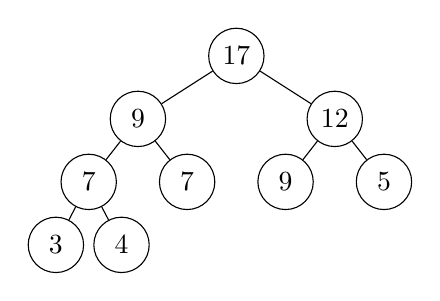
\begin{tikzpicture}[every node/.style={circle,draw,minimum size=2em,inner sep=1},
	baseline={(current bounding box.center)},
	level/.style={level distance=8mm,sibling distance=25mm/#1}]
\node {17} 
child {node {9}
	child {node {7}
		child {node {3}}
		child {node {4}}
		}
	child {node {7}}
	}
child {node {12}
	child {node {9}}
	child {node {5}}
	};
\end{tikzpicture}

[17,9,12,7,7,9,5,3,4]
\end{center}

\subsubsection*{\texttt{insert}}

\noindent Increment ``heapsize'', add element at new index ``heapsize''. Result might violate heap property: ``bubble'' element up (exchange it with its parent) until priority no greater than priority of parent. $\Theta(\textrm{height}) = \Theta(\log n)$ time. For example, \texttt{insert(13)} on previous heap:

\begin{tabular}{c @{ $\rightarrow$ } c @{ $\rightarrow$ } c}

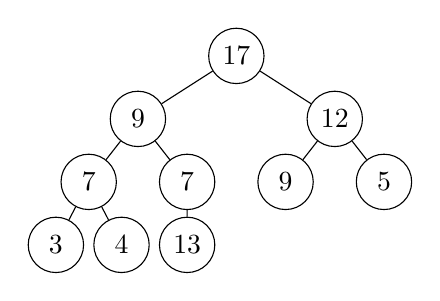
\begin{tikzpicture}[every node/.style={circle,draw,minimum size=2em,inner sep=1},
	baseline={(current bounding box.center)},
	level/.style={level distance=8mm,
	sibling distance=25mm/#1}]
\node {17} 
child {node {9}
	child {node {7}
		child {node {3}}
		child {node {4}}
		}
	child {node {7}
		child {node {13}}
		}
	}
child {node {12}
	child {node {9}}
	child {node {5}}
	};
\end{tikzpicture} & 

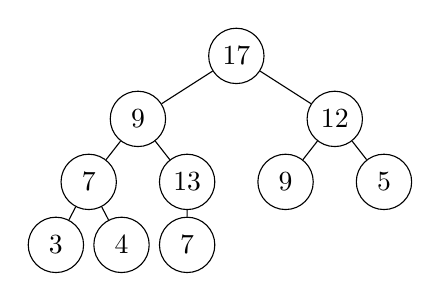
\begin{tikzpicture}[every node/.style={circle,draw,minimum size=2em,inner sep=1},
	baseline={(current bounding box.center)},
	level/.style={level distance=8mm,
	sibling distance=25mm/#1}]
\node {17} 
child {node {9}
	child {node {7}
		child {node {3}}
		child {node {4}}
		}
	child {node {13}
		child {node {7}}
		}
	}
child {node {12}
	child {node {9}}
	child {node {5}}
	};
\end{tikzpicture} &

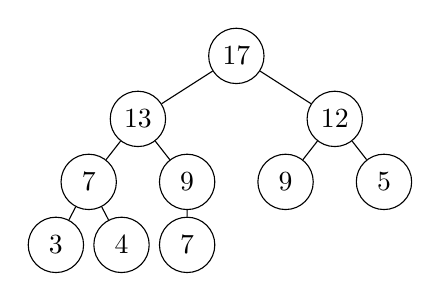
\begin{tikzpicture}[every node/.style={circle,draw,minimum size=2em,inner sep=1},
	baseline={(current bounding box.center)},
	level/.style={level distance=8mm,
	sibling distance=25mm/#1}]
\node {17} 
child {node {13}
	child {node {7}
		child {node {3}}
		child {node {4}}
		}
	child {node {9}
		child {node {7}}
		}
	}
child {node {12}
	child {node {9}}
	child {node {5}}
	};
\end{tikzpicture} \\

[17,9,12,7,7,9,5,3,4,13] & [17,9,12,7,13,9,5,3,4,7] & [17,13,12,7,9,9,5,3,4,7] \\

\end{tabular}

\subsubsection*{\texttt{maximum}}

\noindent Return element at index 1 (if heapsize $\geq$ 1). $\Theta(1)$ time.

\subsubsection*{\texttt{extractMax}}

\noindent Decrement ``heapsize'', remove element at index 1. This leaves ``hole'' at index 1: move element at ``heapsize + 1'' into index 1. Restore heap order by ``percolating down'' (exchange with highest priority child until priority is greater than or equal to both children, or leaf is reached). $\Theta(\log n)$ time. For example, \texttt{extractMax} on previous heap:

\begin{tabular}{c @{ $\rightarrow$ } c @{ $\rightarrow$ } c}

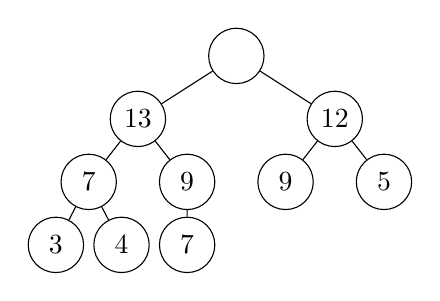
\begin{tikzpicture}[every node/.style={circle,draw,minimum size=2em,inner sep=1},
	baseline={(current bounding box.center)},
	level/.style={level distance=8mm,
	sibling distance=25mm/#1}]
\node { } 
child {node {13}
	child {node {7}
		child {node {3}}
		child {node {4}}
		}
	child {node {9}
		child {node {7}}
		}
	}
child {node {12}
	child {node {9}}
	child {node {5}}
	};
\end{tikzpicture} & 

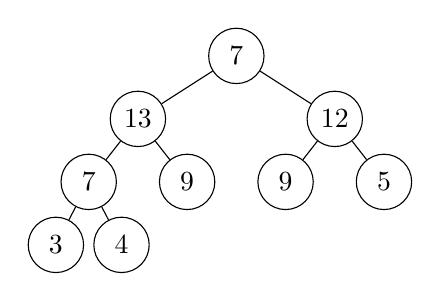
\begin{tikzpicture}[every node/.style={circle,draw,minimum size=2em,inner sep=1},
	baseline={(current bounding box.center)},
	level/.style={level distance=8mm,
	sibling distance=25mm/#1}]
\node {7} 
child {node {13}
	child {node {7}
		child {node {3}}
		child {node {4}}
		}
	child {node {9}}
	}
child {node {12}
	child {node {9}}
	child {node {5}}
	}; 
\end{tikzpicture} & \\

[ ,13,12,7,9,9,5,3,4,7] & [7,13,12,7,9,9,5,3,4] & \\

\end{tabular}

\begin{tabular}{c @{ $\rightarrow$ } c}

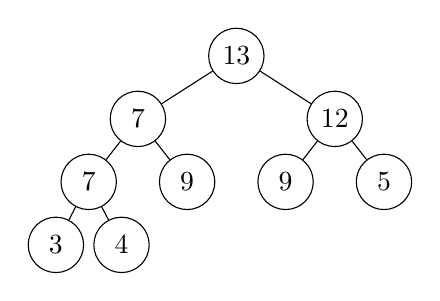
\begin{tikzpicture}[every node/.style={circle,draw,minimum size=2em,inner sep=1},
	baseline={(current bounding box.center)},
	level/.style={level distance=8mm,
	sibling distance=25mm/#1}]
\node {13} 
child {node {7}
	child {node {7}
		child {node {3}}
		child {node {4}}
		}
	child {node {9}}
	}
child {node {12}
	child {node {9}}
	child {node {5}}
	}; 
\end{tikzpicture} &

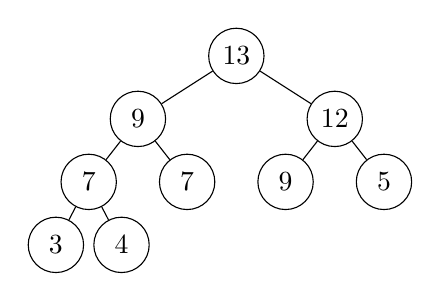
\begin{tikzpicture}[every node/.style={circle,draw,minimum size=2em,inner sep=1},
	baseline={(current bounding box.center)},
	level/.style={level distance=8mm,
	sibling distance=25mm/#1}]
\node {13} 
child {node {9}
	child {node {7}
		child {node {3}}
		child {node {4}}
		}
	child {node {7}}
	}
child {node {12}
	child {node {9}}
	child {node {5}}
	}; 
\end{tikzpicture} \\

[13,7,12,7,9,9,5,3,4] & [13,9,12,7,7,9,5,3,4] \\

\end{tabular}

\subsubsection*{\texttt{increasePriority}}

\noindent Simply bubble element up the heap to restore head order. $\Theta(\log n)$ time. For example, \texttt{increasePriority(4,10)}:

\begin{tabular}{c @{ $\rightarrow$ } c @{ $\rightarrow$ } c}

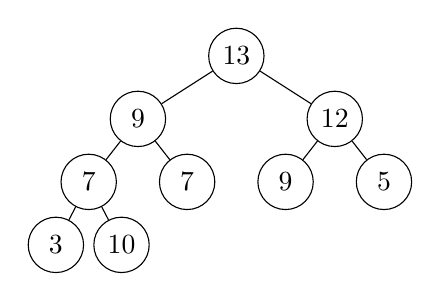
\begin{tikzpicture}[every node/.style={circle,draw,minimum size=2em,inner sep=1},
	baseline={(current bounding box.center)},
	level/.style={level distance=8mm,
	sibling distance=25mm/#1}]
\node {13} 
child {node {9}
	child {node {7}
		child {node {3}}
		child {node {10}}
		}
	child {node {7}}
	}
child {node {12}
	child {node {9}}
	child {node {5}}
	};
\end{tikzpicture} & 

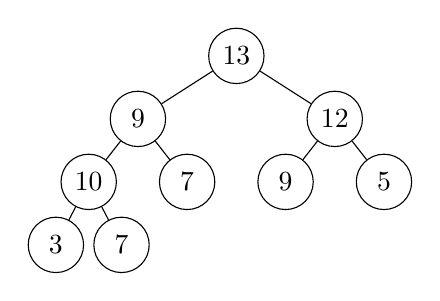
\begin{tikzpicture}[every node/.style={circle,draw,minimum size=2em,inner sep=1},
	baseline={(current bounding box.center)},
	level/.style={level distance=8mm,
	sibling distance=25mm/#1}]
\node {13} 
child {node {9}
	child {node {10}
		child {node {3}}
		child {node {7}}
		}
	child {node {7}}
	}
child {node {12}
	child {node {9}}
	child {node {5}}
	};
\end{tikzpicture} &

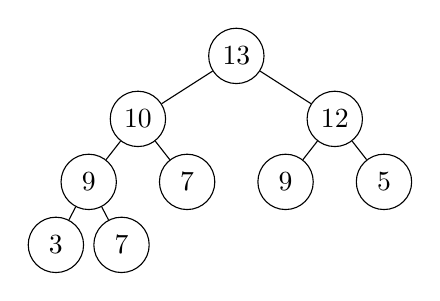
\begin{tikzpicture}[every node/.style={circle,draw,minimum size=2em,inner sep=1},
	baseline={(current bounding box.center)},
	level/.style={level distance=8mm,
	sibling distance=25mm/#1}]
\node {13} 
child {node {10}
	child {node {9}
		child {node {3}}
		child {node {7}}
		}
	child {node {7}}
	}
child {node {12}
	child {node {9}}
	child {node {5}}
	};
\end{tikzpicture} \\

[13,9,12,7,7,9,5,3,10] & [13,9,12,10,7,9,5,3,7] & [13,10,12,9,7,9,5,3,7] \\

\end{tabular}

\end{document}





























